\documentclass{article}

\usepackage{fancyhdr}
\usepackage{extramarks}
\usepackage{amsmath}
\usepackage{amsthm}
\usepackage{amsfonts}
\usepackage{tikz}
\usepackage[plain]{algorithm}
\usepackage{algpseudocode}
\usepackage{mathtools}

\usepackage[utf8]{inputenc}

% Default fixed font does not support bold face
\DeclareFixedFont{\ttb}{T1}{txtt}{bx}{n}{12} % for bold
\DeclareFixedFont{\ttm}{T1}{txtt}{m}{n}{12}  % for normal

% Custom colors
\usepackage{color}
\definecolor{deepblue}{rgb}{0,0,0.5}
\definecolor{deepred}{rgb}{0.6,0,0}
\definecolor{deepgreen}{rgb}{0,0.5,0}

\usepackage{listings}

% Python style for highlighting
\newcommand\pythonstyle{\lstset{
language=Python,
basicstyle=\ttm,
morekeywords={self},              % Add keywords here
keywordstyle=\ttb\color{deepblue},
emph={MyClass,__init__},          % Custom highlighting
emphstyle=\ttb\color{deepred},    % Custom highlighting style
stringstyle=\color{deepgreen},
frame=tb,                         % Any extra options here
showstringspaces=false
}}


% Python environment
\lstnewenvironment{python}[1][]
{
\pythonstyle
\lstset{#1}
}
{}

\usetikzlibrary{automata,positioning}

%
% Basic Document Settings
%

\topmargin=-0.45in
\evensidemargin=0in
\oddsidemargin=0in
\textwidth=6.5in
\textheight=9.0in
\headsep=0.25in

\linespread{1.1}

\pagestyle{fancy}
\lhead{\hmwkAuthorName}
\chead{\hmwkClass\ (\hmwkClassInstructor\ \hmwkClassTime): \hmwkTitle}
\rhead{\firstxmark}
\lfoot{\lastxmark}
\cfoot{\thepage}

\renewcommand\headrulewidth{0.4pt}
\renewcommand\footrulewidth{0.4pt}

\setlength\parindent{0pt}

%
% Create Problem Sections
%

\newcommand{\enterProblemHeader}[1]{
    \nobreak\extramarks{}{Problem \arabic{#1} continued on next page\ldots}\nobreak{}
    \nobreak\extramarks{Problem \arabic{#1} (continued)}{Problem \arabic{#1} continued on next page\ldots}\nobreak{}
}

\newcommand{\exitProblemHeader}[1]{
    \nobreak\extramarks{Problem \arabic{#1} (continued)}{Problem \arabic{#1} continued on next page\ldots}\nobreak{}
    \stepcounter{#1}
    \nobreak\extramarks{Problem \arabic{#1}}{}\nobreak{}
}

\setcounter{secnumdepth}{0}
\newcounter{partCounter}
\newcounter{homeworkProblemCounter}
\setcounter{homeworkProblemCounter}{1}
\nobreak\extramarks{Problem \arabic{homeworkProblemCounter}}{}\nobreak{}

%
% Homework Problem Environment
%
% This environment takes an optional argument. When given, it will adjust the
% problem counter. This is useful for when the problems given for your
% assignment aren't sequential. See the last 3 problems of this template for an
% example.
%
\newenvironment{homeworkProblem}[1][-1]{
    \ifnum#1>0
        \setcounter{homeworkProblemCounter}{#1}
    \fi
    \section{Section \arabic{homeworkProblemCounter}}
    \setcounter{partCounter}{1}
    \enterProblemHeader{homeworkProblemCounter}
}{
    \exitProblemHeader{homeworkProblemCounter}
}

%
% Homework Details
%   - Title
%   - Due date
%   - Class
%   - Section/Time
%   - Instructor
%   - Author
%

\newcommand{\hmwkTitle}{Assignment 2\ \#2}
\newcommand{\hmwkDueDate}{\today}
\newcommand{\hmwkClass}{Investigating Dynamic System}
\newcommand{\hmwkClassTime}{Section A}
\newcommand{\hmwkClassInstructor}{Professor J}
\newcommand{\hmwkAuthorName}{\textbf{V} \and \textbf{U}}

%
% Title Page
%

\title{
    \vspace{2in}
    \textmd{\textbf{\hmwkClass:\ \hmwkTitle}}\\
    \normalsize\vspace{0.1in}\small{Due\ on\ \hmwkDueDate\ at 3:10pm}\\
    \vspace{0.1in}\large{\textit{\hmwkClassInstructor\ \hmwkClassTime}}
    \vspace{3in}
}

\author{\hmwkAuthorName}
\date{}

\renewcommand{\part}[1]{\textbf{\large Part \Alph{partCounter}}\stepcounter{partCounter}\\}

%
% Various Helper Commands
%

% Useful for algorithms
\newcommand{\alg}[1]{\textsc{\bfseries \footnotesize #1}}

% For derivatives
\newcommand{\deriv}[1]{\frac{\mathrm{d}}{\mathrm{d}x} (#1)}

% For partial derivatives
\newcommand{\pderiv}[2]{\frac{\partial}{\partial #1} (#2)}

% Integral dx
\newcommand{\dx}{\mathrm{d}x}

% Alias for the Solution section header
\newcommand{\solution}{\textbf{\large Solution}}

% Probability commands: Expectation, Variance, Covariance, Bias
\newcommand{\E}{\mathrm{E}}
\newcommand{\Var}{\mathrm{Var}}
\newcommand{\Cov}{\mathrm{Cov}}
\newcommand{\Bias}{\mathrm{Bias}}

\begin{document}

\maketitle

\pagebreak

\section{Introduction}
	A study shows that a ball falling in a gravitational field in absense of friction conforms the a 
	differential equation. In this study, a variety of properties of the system of equation have been discovered. 
	Imagin a ball rolling around in a basin of height $h = h(x, y)$, with $\mathbf{x}(t) = (x(t), y(t))$ be two-dimensional vector describing the position of the ball at $t$.
	The ball is accelerated by gravity and then its motion forms the following differential equation
	
	\begin{equation}
		\begin{cases}
			\ddot{x} &= -\frac{\partial h}{\partial x}, \\
			\ddot{y} &= -\frac{\partial h}{\partial y}
		\end{cases}
	\end{equation}

	We plugin $h(x, y) = \frac{1}{2}(x^2+y^2) + x^2y - \frac{1}{3}y^3$
	\begin{equation}
		\begin{cases}
			\ddot{x} &= -x - 2xy, \\
			\ddot{y} &= -y -x^2+y^2
		\end{cases}
	\end{equation}

	and

	\begin{equation}
		\begin{cases}
			\ddot{x} = \frac{\partial h}{\partial x}, \\
			\ddot{y} = \frac{\partial h}{\partial y}
		\end{cases}
	\end{equation}

\section*{Derivation}
	One observation is that 
	\begin{align*}
		\ddot{x} &= -\frac{\partial h}{\partial x} \\
		         &= \partial_x\left(-\frac{1}{2}x^2\right) +  \partial_x\left(-\frac{1}{2}y^2\right) + \partial_x(-xy^2)+\partial_x(-\frac{1}{3}y^3) \\ 
				 &= -x + 0 - 2xy + 0 \\
				 &= -x -2xy
	\end{align*}

	\begin{align*}
		\ddot{y} &= \partial_y\left(-\frac{1}{2}x^2\right) +  \partial_y\left(-\frac{1}{2}y^2\right) + \partial_x(-xy^2)+\partial_y(-\frac{1}{3}y^3) \\
				 &= -y + 0 -x^2 + y^2\\
				 &= -y-x^2+y^2
	\end{align*}

	\subsection*{Constant energy function}
	We have that the energy function
	\[E = \frac{1}{2}(\dot{x}^2 + \dot{y}^2) + h(x,y)\]
	is constant

	we can derive this result by chain rule, and from the result above

	\begin{align*}
		\frac{dE}{dt} &= \frac{1}{2}\left(\frac{d\dot{x}^2}{dt} + \frac{d\dot{y}^2}{dt} \right) + \frac{dh}{dt}\\
					  &= \frac{1}{2}(2\dot{x}\ddot{x} + 2\dot{y}\ddot{y}) + \frac{\partial h}{\partial x}\frac{dx}{dt} + \frac{\partial h}{\partial y}\frac{dy}{dt}\\
					  &= \dot{x}\ddot{x} + \dot{y}\ddot{y} + (-\ddot{x}\dot{x}) + (-\ddot{y}\dot{y}) \\
					  &= (\dot{x}\ddot{x} - \ddot{x}\ddot{x}) + (\dot{y}\ddot{y} - \ddot{y}\dot{y}) \\
					  &= 0
	\end{align*}

$h$ has four stationary points, we can obtain them by solving the system of equations

\begin{equation}
	\begin{cases}
		\partial_x h(x,y) &= x + 2xy = 0 \\
		\partial_y h(x,y) &= y + x^2 - y^2 = 0
	\end{cases}
\end{equation}

we have 

\begin{equation}
	\begin{cases}
		x(1+2y) &= 0 \\
		y + x^2 - y^2 &= 0
	\end{cases}
\end{equation}

\begin{equation}
	\begin{cases}
		x = 0 \\
		y = 0
	\end{cases}
\end{equation}
\begin{equation}
	\begin{cases}
		x = 0 \\
		y = 1
	\end{cases}
\end{equation}
\begin{equation}
	\begin{cases}
		x = \frac{\sqrt{3}}{2} \\
		y = -\frac{1}{2}
	\end{cases}
\end{equation}
\begin{equation}
	\begin{cases}
		x = -\frac{\sqrt{3}}{2} \\
		y = -\frac{1}{2}
	\end{cases}
\end{equation}

Let \begin{align*}
		D(a, b) &= h_{xx}(a, b)h_{yy}(a, b) - h_{xy}^{2}(a, b) = (1 + 2y)(1 - 2y) - 4x^2 \\ 
				&= 1- 4y^2 - 4x^2
	\end{align*}

According to the criteria of stationary point, which is involving Hessian matrix. We have the following results.
\begin{enumerate}
	\item Since $D(0, 0) = 1 > 0$ and $h_{xx}(0,0) = 1 > 0$, so $(0,0)$ is local minimum
	\item Since $D(0, 1) = -3 < 0$, so $(0, 1)$ is saddle point.
	\item Since $D\left(-\frac{\sqrt{3}}{2}, -\frac{1}{2}\right) = D\left(\frac{\sqrt{3}}{2}, -\frac{1}{2}\right) = -3 < 0$ so $\left(\pm\frac{\sqrt{3}}{2}, -\frac{1}{2}\right)$ are saddle points as well.
\end{enumerate}

with $(0,0)$ being minimum point, and others being saddle points

The second order ODEs can be rewritten as a system of first order ODEs.
\begin{equation}
	\begin{cases}
		\dot{x} = p_x\\
		\dot{y} = p_y\\
		\dot{p_x} = -x - 2xy \\
		\dot{p_y} = -y -x^2 + y^2 
	\end{cases}
\end{equation}

\pagebreak

\section{Contour Graph}
Contour Plot.

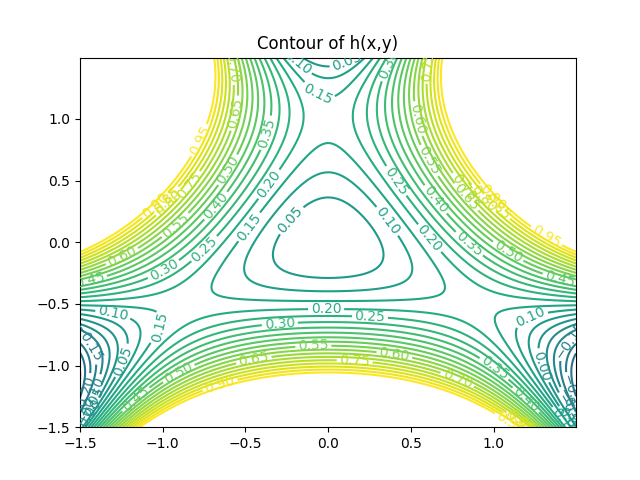
\includegraphics[scale=0.5]{./Contour.png}

We have some observation according to the graph.
The value of contour that joins three stationary point is approximately 0.15 by the look of the graph. In theory it is $\frac{1}{6}\approx 1.67$
We've found that a central basin is at $(0, 0)$.
The graph is symmetric with regard to the axis $x = 0$.
The contours colored with yellow have larger values, thus representing mountains.
The green contours in between those yello mountains are valleys in this sense.

\section{Trajectory graph}
	This shows the Trajectory when $x_0 = 0.3, y_0 = 0, p_x = 0, p_y = 0.2$
	The trajectory is seemingly symmetric with
	regard to the origin and the $y$-axis. with $-0.5\le x \le 0.6$, and $-0.28 \le y \le 0.28$.

	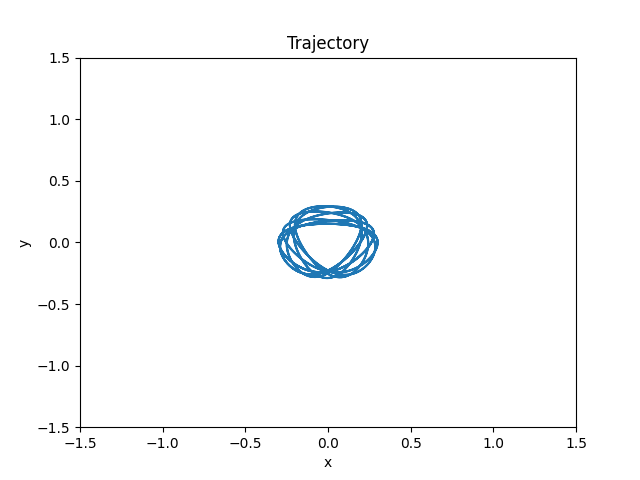
\includegraphics[scale=0.5]{./Trajectory.png} 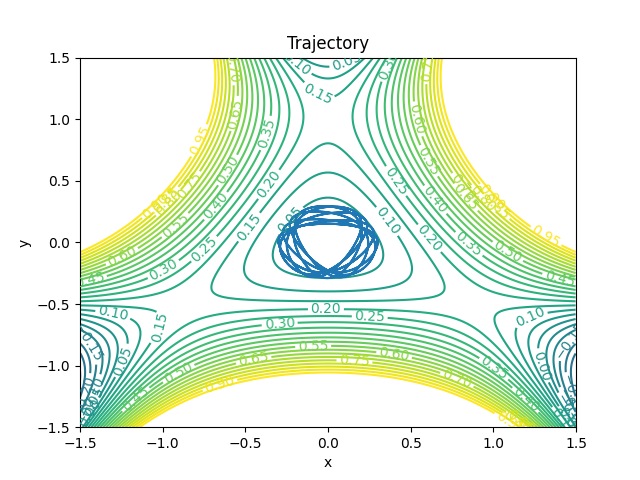
\includegraphics[scale=0.5]{./Trajectory_with_contour.png}

	This shows the trajectory $x_0 = 0.5, y_0 = 0, p_x = 0, p_y = 0.3$. The trajectory is seemingly symmetric with
	regard to the origin and the $y$-axis with $-0.5\le y \le 0.7$, and $-0.6 \le x \le 0.6$.

	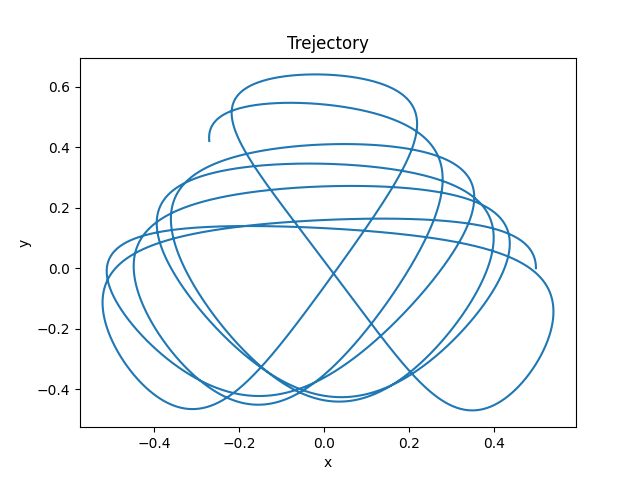
\includegraphics[scale=0.5]{./Ject6000.png}
	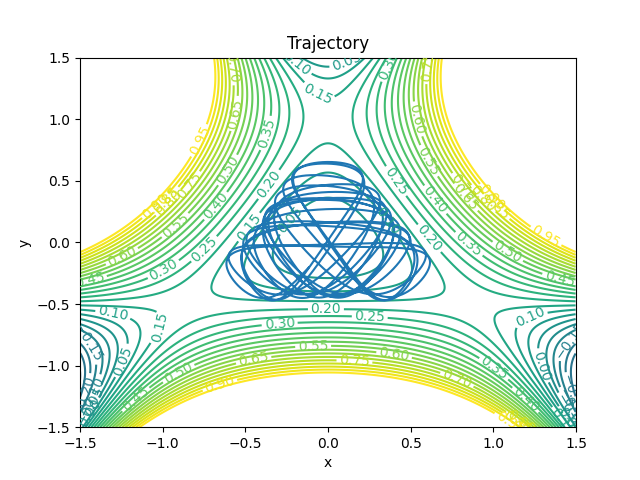
\includegraphics[scale=0.5]{./Ject6000_with_contour.png}

	This graph shows the trajectory with initial values $x_0 = -0.2, y_0 = 0, p_x = 0, p_y = -0.5$. This trajectory shows less symmetricity than
	the previous 2 graph. This can be the cause of negative value of $x_0$, and $p_y$.


	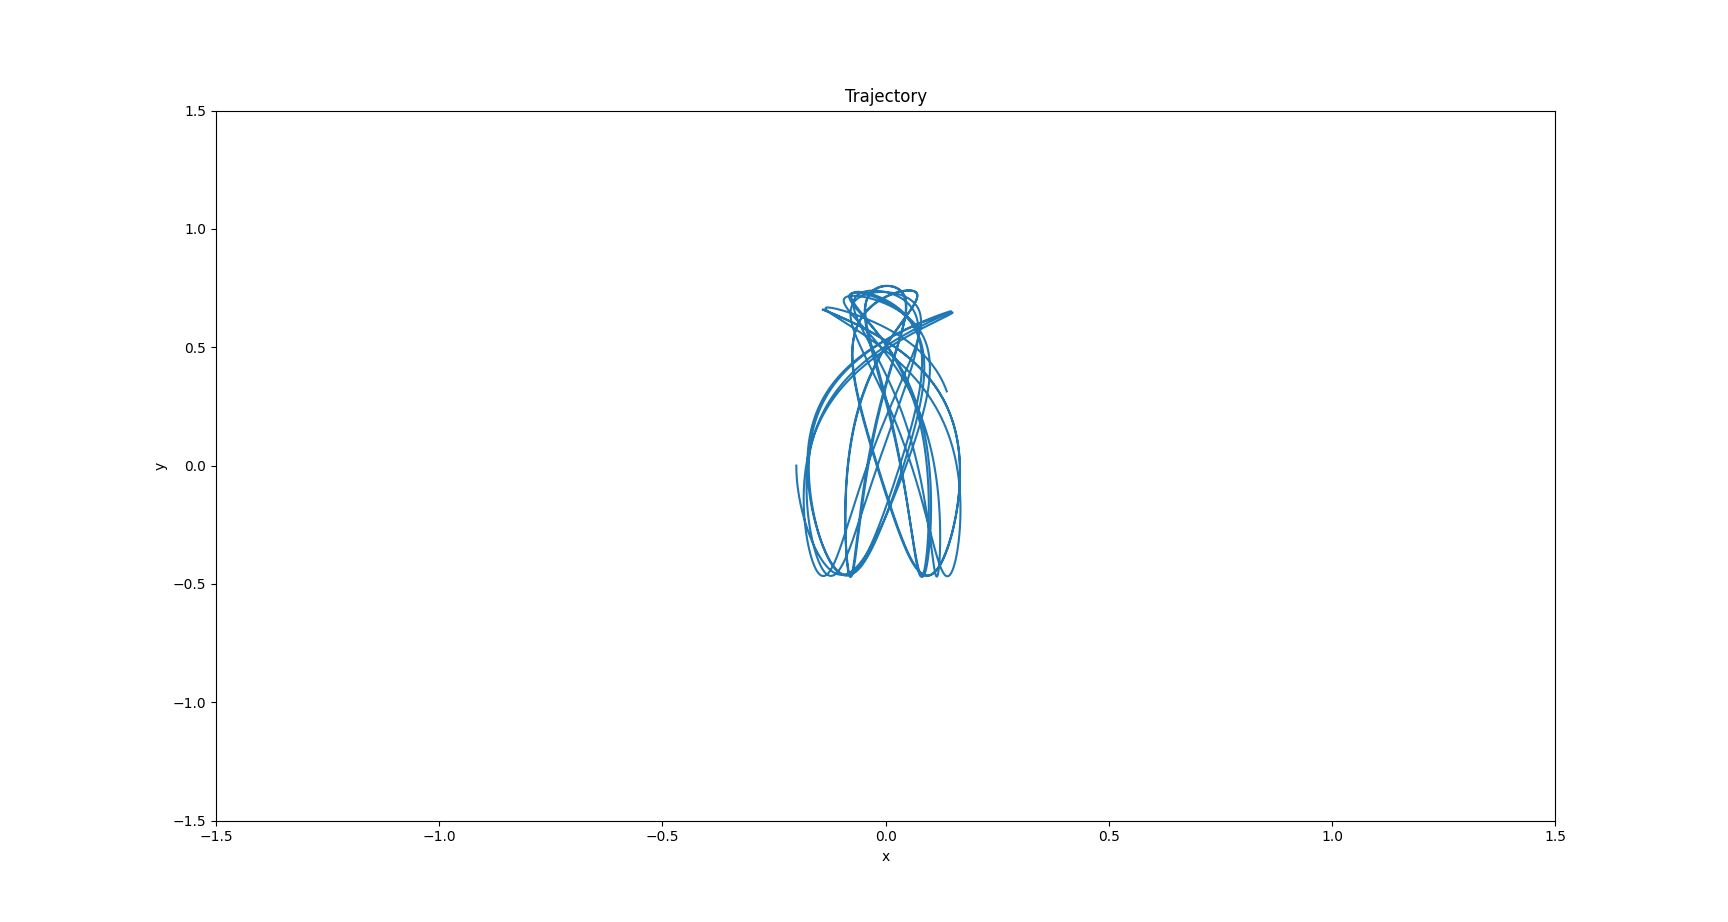
\includegraphics[scale=0.3, width=300]{./Trajectory2.png}
	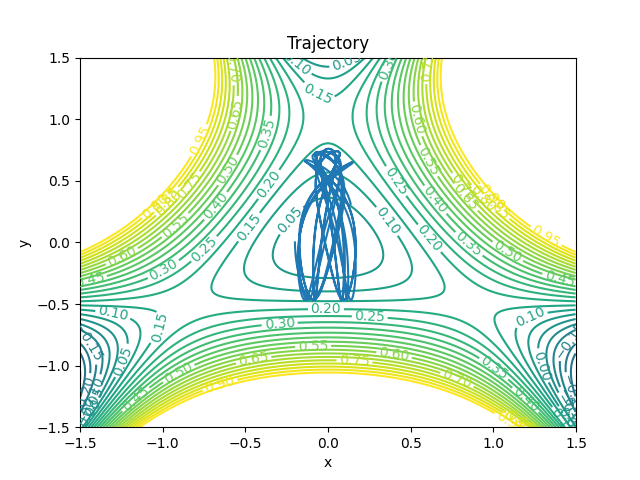
\includegraphics[scale=0.5]{./Trajectory2_with_contour.png}

\section{Escape with exit}
	We now investigate the initial values such that the corresponding differential equation gives a escaping trajectory.
	That means a trajectory will eventually diverge into infinity(positive or negative). Again we are fixing the value $y$ and $p_x$, but changing $x$, and $p_y$.
	We've dicovered that if we choose $x = 0.6, y = 0, p_x = 0.0, p_y = 0.6$, we would obtain a desired trajectory as followed.

	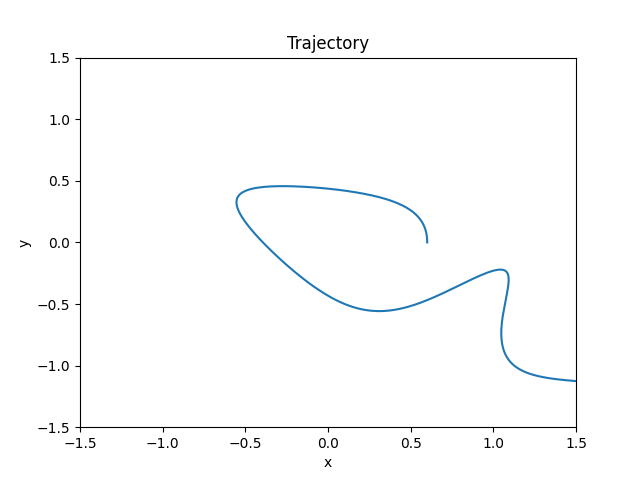
\includegraphics[scale=0.5]{./escape.png}

	We put the contour graph together with the trajectory plot. As it shows, the trajectory starts at the origin. And then it climb up to the hill on the left side,
	making a left turn like a parabola, 
	coming near and exiting the stationary point $(0,1)$, ending up going to infinity where $y = \infty$.

	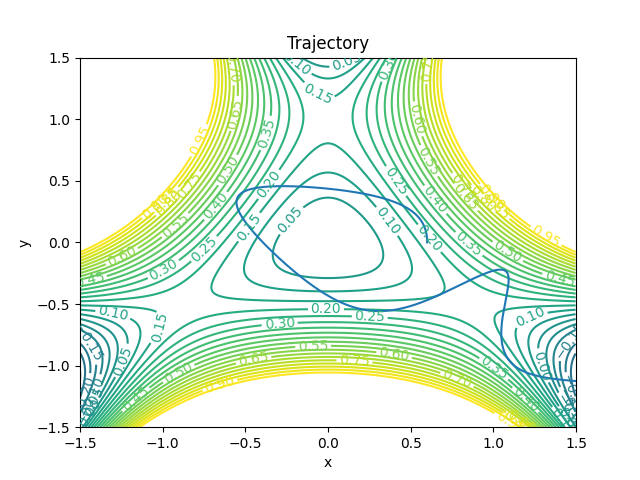
\includegraphics[scale=0.5]{./escape_trajectory_with_contour.png}

	We want to investigate the situation of each point, in which case whether this point will exit through which stationary point, or stay in 
	the basin forever. 
	
	The following graph shows the distribution of whether each initial point of $(x_0, py_0)$
	is a escaping trajectory with which exit or wandering around the basin. And a werid scenario is that there is blue dots in the area of green dots.
	which making the boundary irregular. 
	
	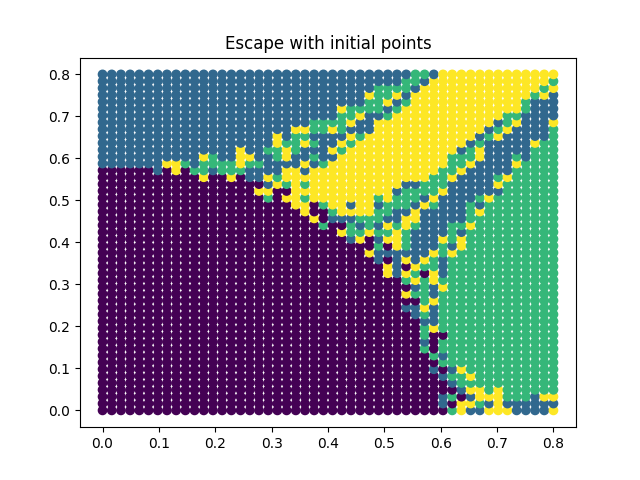
\includegraphics[scale=0.5]{./escape_dist.png}
	

	where the purple colour denotes trajectory around the basin;
	the blue/yellow/green colours denote the trajectories with exit 1,2,3;

	It looks like that the boundary of the basin is a circle with radius $0.5$. 

\section{Conclusion}
In this assignment the study the various property of this trajectory equation has been conduct.
First off, we had study the theoretical property of the differential equation. Several tationry points have be been found.
And then we had concluded if a trajectory could escape the basin.

\end{document}